\documentclass[12pt,fleqn,answers]{exam}
\usepackage{pifont}
\usepackage{dingbat}
\usepackage{amsmath,amssymb}
\usepackage{epsfig}
\usepackage[]{hyperref}
\usepackage{geometry}
\usepackage[]{graphicx}
\geometry{letterpaper, margin=0.5in}
\addpoints
\boxedpoints
\pointsinmargin
\pointname{pts}

\usepackage[activate={true,nocompatibility},final,tracking=true,kerning=true,factor=1100,stretch=10,shrink=10]{microtype}
\usepackage[american]{babel}
%\usepackage[T1]{fontenc}
\usepackage{fourier}
\usepackage{isomath}
\usepackage{upgreek,amsmath}
\usepackage{amssymb}

\newcommand{\dotprod}{\, {\scriptzcriptztyle
    \stackrel{\bullet}{{}}}\,}

\newcommand{\reals}{\mathbf{R}}
\newcommand{\lub}{\mathrm{lub}} 
\newcommand{\glb}{\mathrm{glb}} 
\newcommand{\complex}{\mathbf{C}}
\newcommand{\dom}{\mbox{dom}}
\newcommand{\cover}{{\mathcal C}}
\newcommand{\integers}{\mathbf{Z}}
\newcommand{\vi}{\, \mathbf{i}}
\newcommand{\vj}{\, \mathbf{j}}
\newcommand{\vk}{\, \mathbf{k}}
\newcommand{\bi}{\, \mathbf{i}}
\newcommand{\bj}{\, \mathbf{j}}
\newcommand{\bk}{\, \mathbf{k}}
\DeclareMathOperator{\Arg}{\mathrm{Arg}}
\DeclareMathOperator{\Ln}{\mathrm{Ln}}
\newcommand{\imag}{\, \mathrm{i}}

\usepackage{graphicx}
\newcommand\AM{{\sc am}}
\newcommand\PM{{\sc pm}}
     
\newcommand{\quiz}{5}
\newcommand{\term}{Fall}
\newcommand{\due}{Saturday 1 October  at 11:59 \PM}
\begin{document}
\large
\vspace{0.1in}
\noindent\makebox[3.0truein][l]{{\bf MATH 460}}
{\bf Name:}  \\
\noindent \makebox[3.0truein][l]{\bf Homework   \quiz, \term \/ \the\year}
%{\bf Row:}\hrulefill\
\vspace{0.1in}

\begin{quote}
    \fbox{I have neither given nor received unauthorized assistance on this assignment.}
    \end{quote}
\noindent  Homework    \quiz\/  has questions 1 through  \numquestions \/ with a total of  \numpoints\/  points.   
Neatly \textbf{handwrite your solutions}, digitize your work, and turn it into Canvas. You do \textbf{not} need to 
use  La\TeX\,  for this assignment. This work is due \emph{\due}.

\vspace{0.1in}

%\noindent{\textbf{Link to your Overleaf work: }}\url{XXX}

\begin{questions} 

\question[5] Show that \(\left( \forall x \in \reals \right) \left(\max(0,x) = \frac{x+|x|}{2} \right) \).
Likely you will want to consider the cases $x < 0$ and $x \geq 0$ separately.

\begin{solution}  We'll consider the cases $x < 0$ and $x \geq 0$ 
    separately. For $x < 0$, we have
    \begin{align*}
        \frac{x+|x|}{2} &= \frac{x-x}{2}, &\mbox{(simplify absolute value)} \\
                        &= 0, &\mbox{(algebra)} \\
                        &= \max(0,x). &\mbox{($x < 0$)} 
    \end{align*}
    For $x \geq 0$, we have
    \begin{align*}
        \frac{x+|x|}{2} &= \frac{x+x}{2}, &\mbox{(simplify absolute value)} \\
                        &= x, &\mbox{(algebra)} \\
                        &= \max(0,x). &\mbox{($x \geq 0$)} 
    \end{align*}
\end{solution}

\question[5] Let $F$ be a convergent sequence. Show that the sequence 
\(k \in \integers_{\geq 0} \mapsto \max(F_k,0)\) converges.
\textbf{Hint:} Use the result of Question 1. 

\begin{solution}  Let's define \(G = k \in \integers_{\geq 0} \mapsto \max(F_k,0)\).
    Alternatively \(G = \frac{F  + |F|}{2}\). Since $F$ converges,
    so does $|F|$. That makes $G$ a linear combination
    of convergent sequences, so $G$ converges.



\end{solution}


\question Define 
\(\displaystyle
    H = n \in \integers_{> 0} \mapsto \sum_{k=1}^n \frac{1}{k}.
\)

\begin{parts}

    \part[5] Use the fact that 
    \(\displaystyle
        \left(\forall x \in \reals_{\geq 1}\right)
         \left(\ln(x+1) - \ln(x) \leq \frac{1}{x} \right)
    \)
    to show that the sequence $H$ is not bounded above (and consequently does 
    not converge). To do this, you will use some standard calculus facts
    about telescoping sums and about the natural logarithm. One fact that you might use is the fact
    that the natural logarithm is not bounded above.
    \begin{solution}  Let $ n \in \integers_{> 0}$. We have
        \begin{align*}
            H_n &= \sum_{k=1}^n \frac{1}{k}, &\mbox{(definiton)}\\
                &\geq \sum_{k=1}^n \ln(k+1) - \ln(k), &\mbox{(given fact)}\\
                &= \ln(n+1) - \ln(1), &\mbox{(telescoping sum)}\\
                &= \ln(n+1). &\mbox{(simplifcation)}\\
        \end{align*}
        Since the natural logarithm isn't bounded above, neither is the
        sequence $H$. Thus $H$ diverges.
         
    \end{solution}

    \part[5] Show that 
    \(
        \left( \forall \, \varepsilon \in \reals_{>0} \right)
        \left(\exists \, n \in \integers \right)
        \left(\forall \, k \in \integers_{> n}\right)
        \left(|H_{k+1} - H_k| < \varepsilon\right)
    \).
\begin{solution}  
    Let $\varepsilon \in \reals_{>0} $. Choose 
    $n = \lceil \frac{1}{\varepsilon} \rceil$. 
    Thus $n \in \integers$ as required. Let $k \in \integers_{>n}$.
    We have
    \[
        |H_{k+1} - H_k| = |\frac{1}{k+1}| < \frac{1}{n}
        = \frac{1}{\lceil \frac{1}{\varepsilon} \rceil}
        \leq  \frac{1}{\frac{1}{\varepsilon}}.
        = \varepsilon.
    \]
\end{solution}
    \part[5] Show that the sequence $H$ is not Cauchy.
    \begin{solution}  
        Since $H$ diverges, it is not Cauchy.
    \end{solution}

\part [5] Draw a graph that shows that
the fact
\(\displaystyle
\left(\forall x \in \reals_{\geq 1}\right)
 \left(\ln(x+1) - \ln(x) \leq \frac{1}{x} \right)
\)
is due to the fact that the natural logarithm function is
concave down. \textbf{Hint:} For the graph \mbox{$y = \ln(x)$}
and a positive number $k$, show the tangent line at the point 
\mbox{$(x=k, y=\ln(k))$} and the 
secant line through the points \mbox{$(x=k, y=\ln(k))$} and 
$(x=k+1, y=\ln(k+1))$.

\end{parts}

\begin{solution}
It's not what I had in mind, but one graphical method is to 
graph both $y = \ln(x+1) - \ln(x)$ and $y = 1/x$ together 
and compare them. Here the red graph is $y = \ln(x+1) - \ln(x)$
and the blue graph is $y = 1/x$ 

\begin{center}
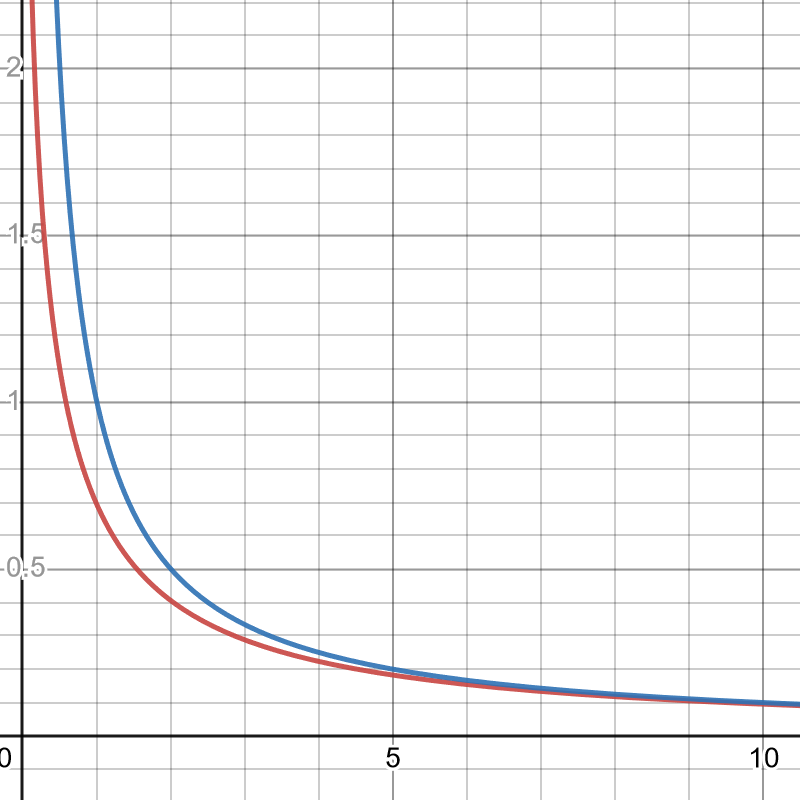
\includegraphics[scale=0.2]{desmos-graph(11).png}
\end{center}
\end{solution}

\end{questions}



\end{document}